\section{Procedure and results}\label{sec: procedure}
Besides the experimentel procedure, this section presents as main results the
absorption spectrum of rubidium. Therefore, the setup shown in figure~\ref{fig: setup}
is used. Before an examination of the spectrum is possible, the laser system has to be
adjust correctly.

To operate the setup properly, the rubidium gas cell must be heated
continiously to $\SI{50}{\degreeCelsius}$. During the heating process, an infrared display
card is inserted in the path of the laser beam. The diode current is increased slowly until a
light spot is visible on the display card. Therefore, a camera is used.
Depending on the current, two emission modes of the laser are observable as presented in 
figure~\ref{fig: emission_modes}.
\begin{figure}
  \centering
      \begin{subfigure}{0.48\textwidth}
          \centering
          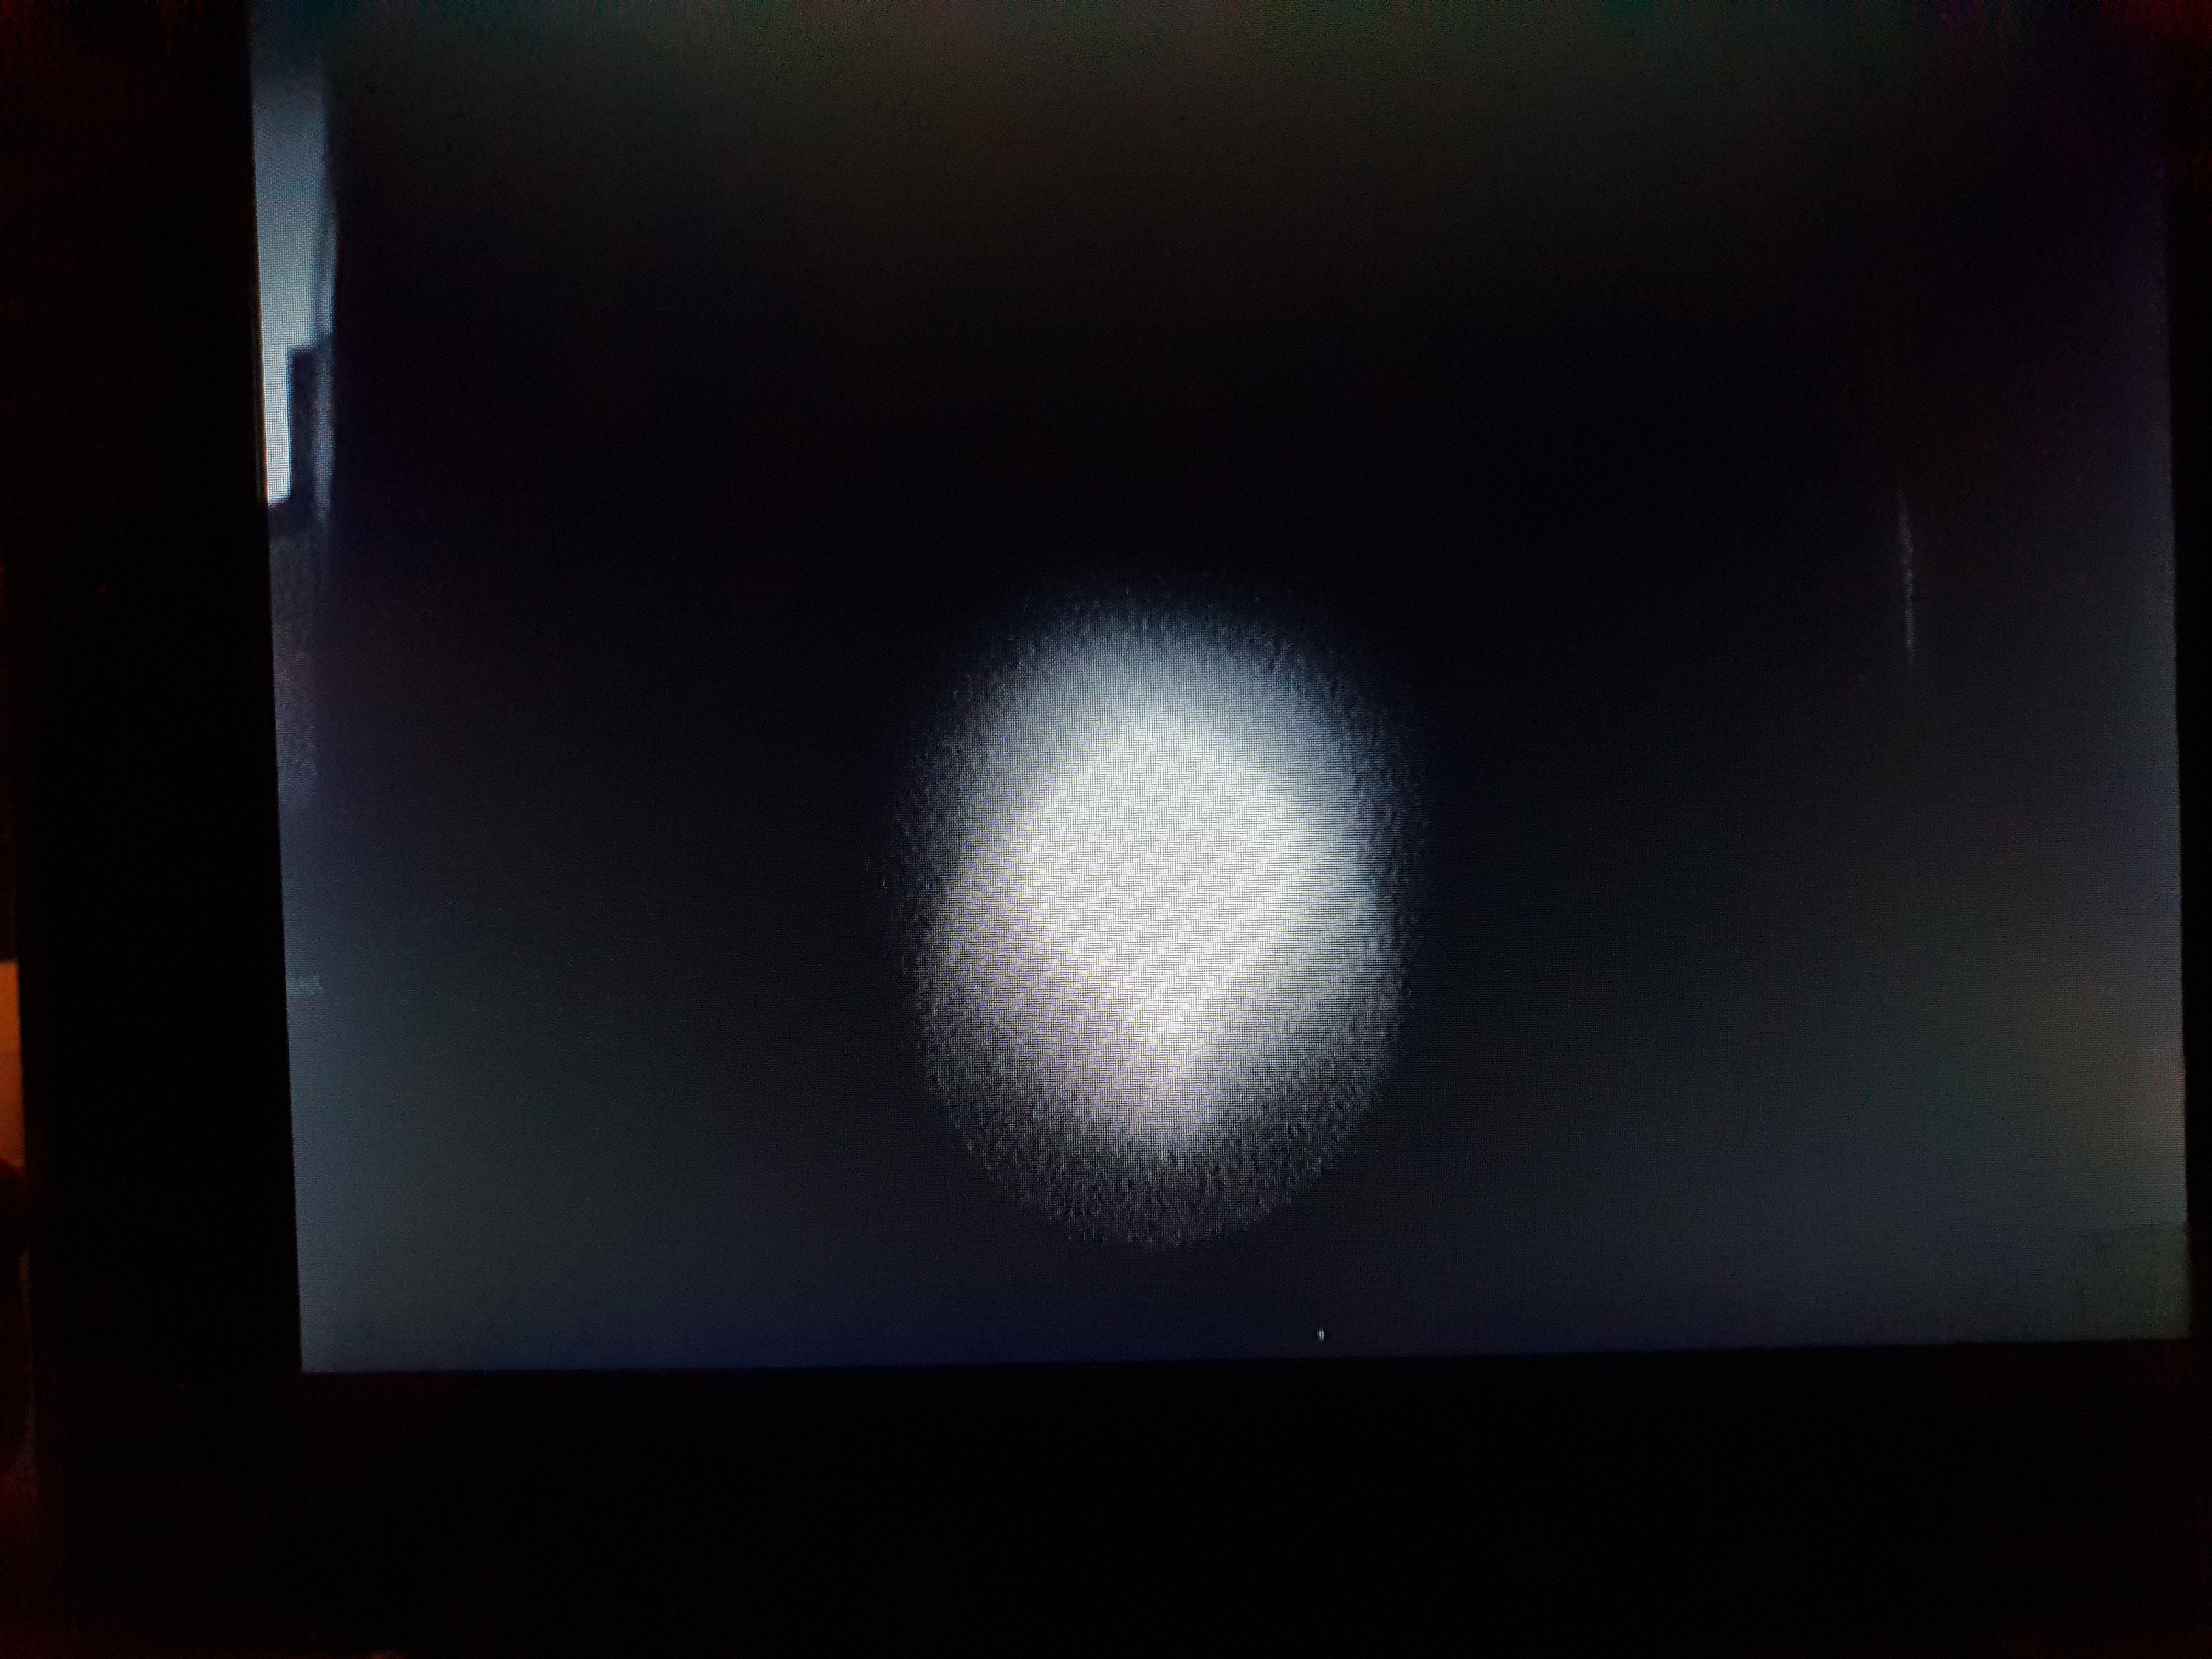
\includegraphics[width = \textwidth]{./content/images/diodelaser_not_lasering.jpg}
          \caption{Not lasing.}
          \label{fig:not_lasering}
      \end{subfigure}
      \begin{subfigure}{0.48\textwidth}
          \centering
          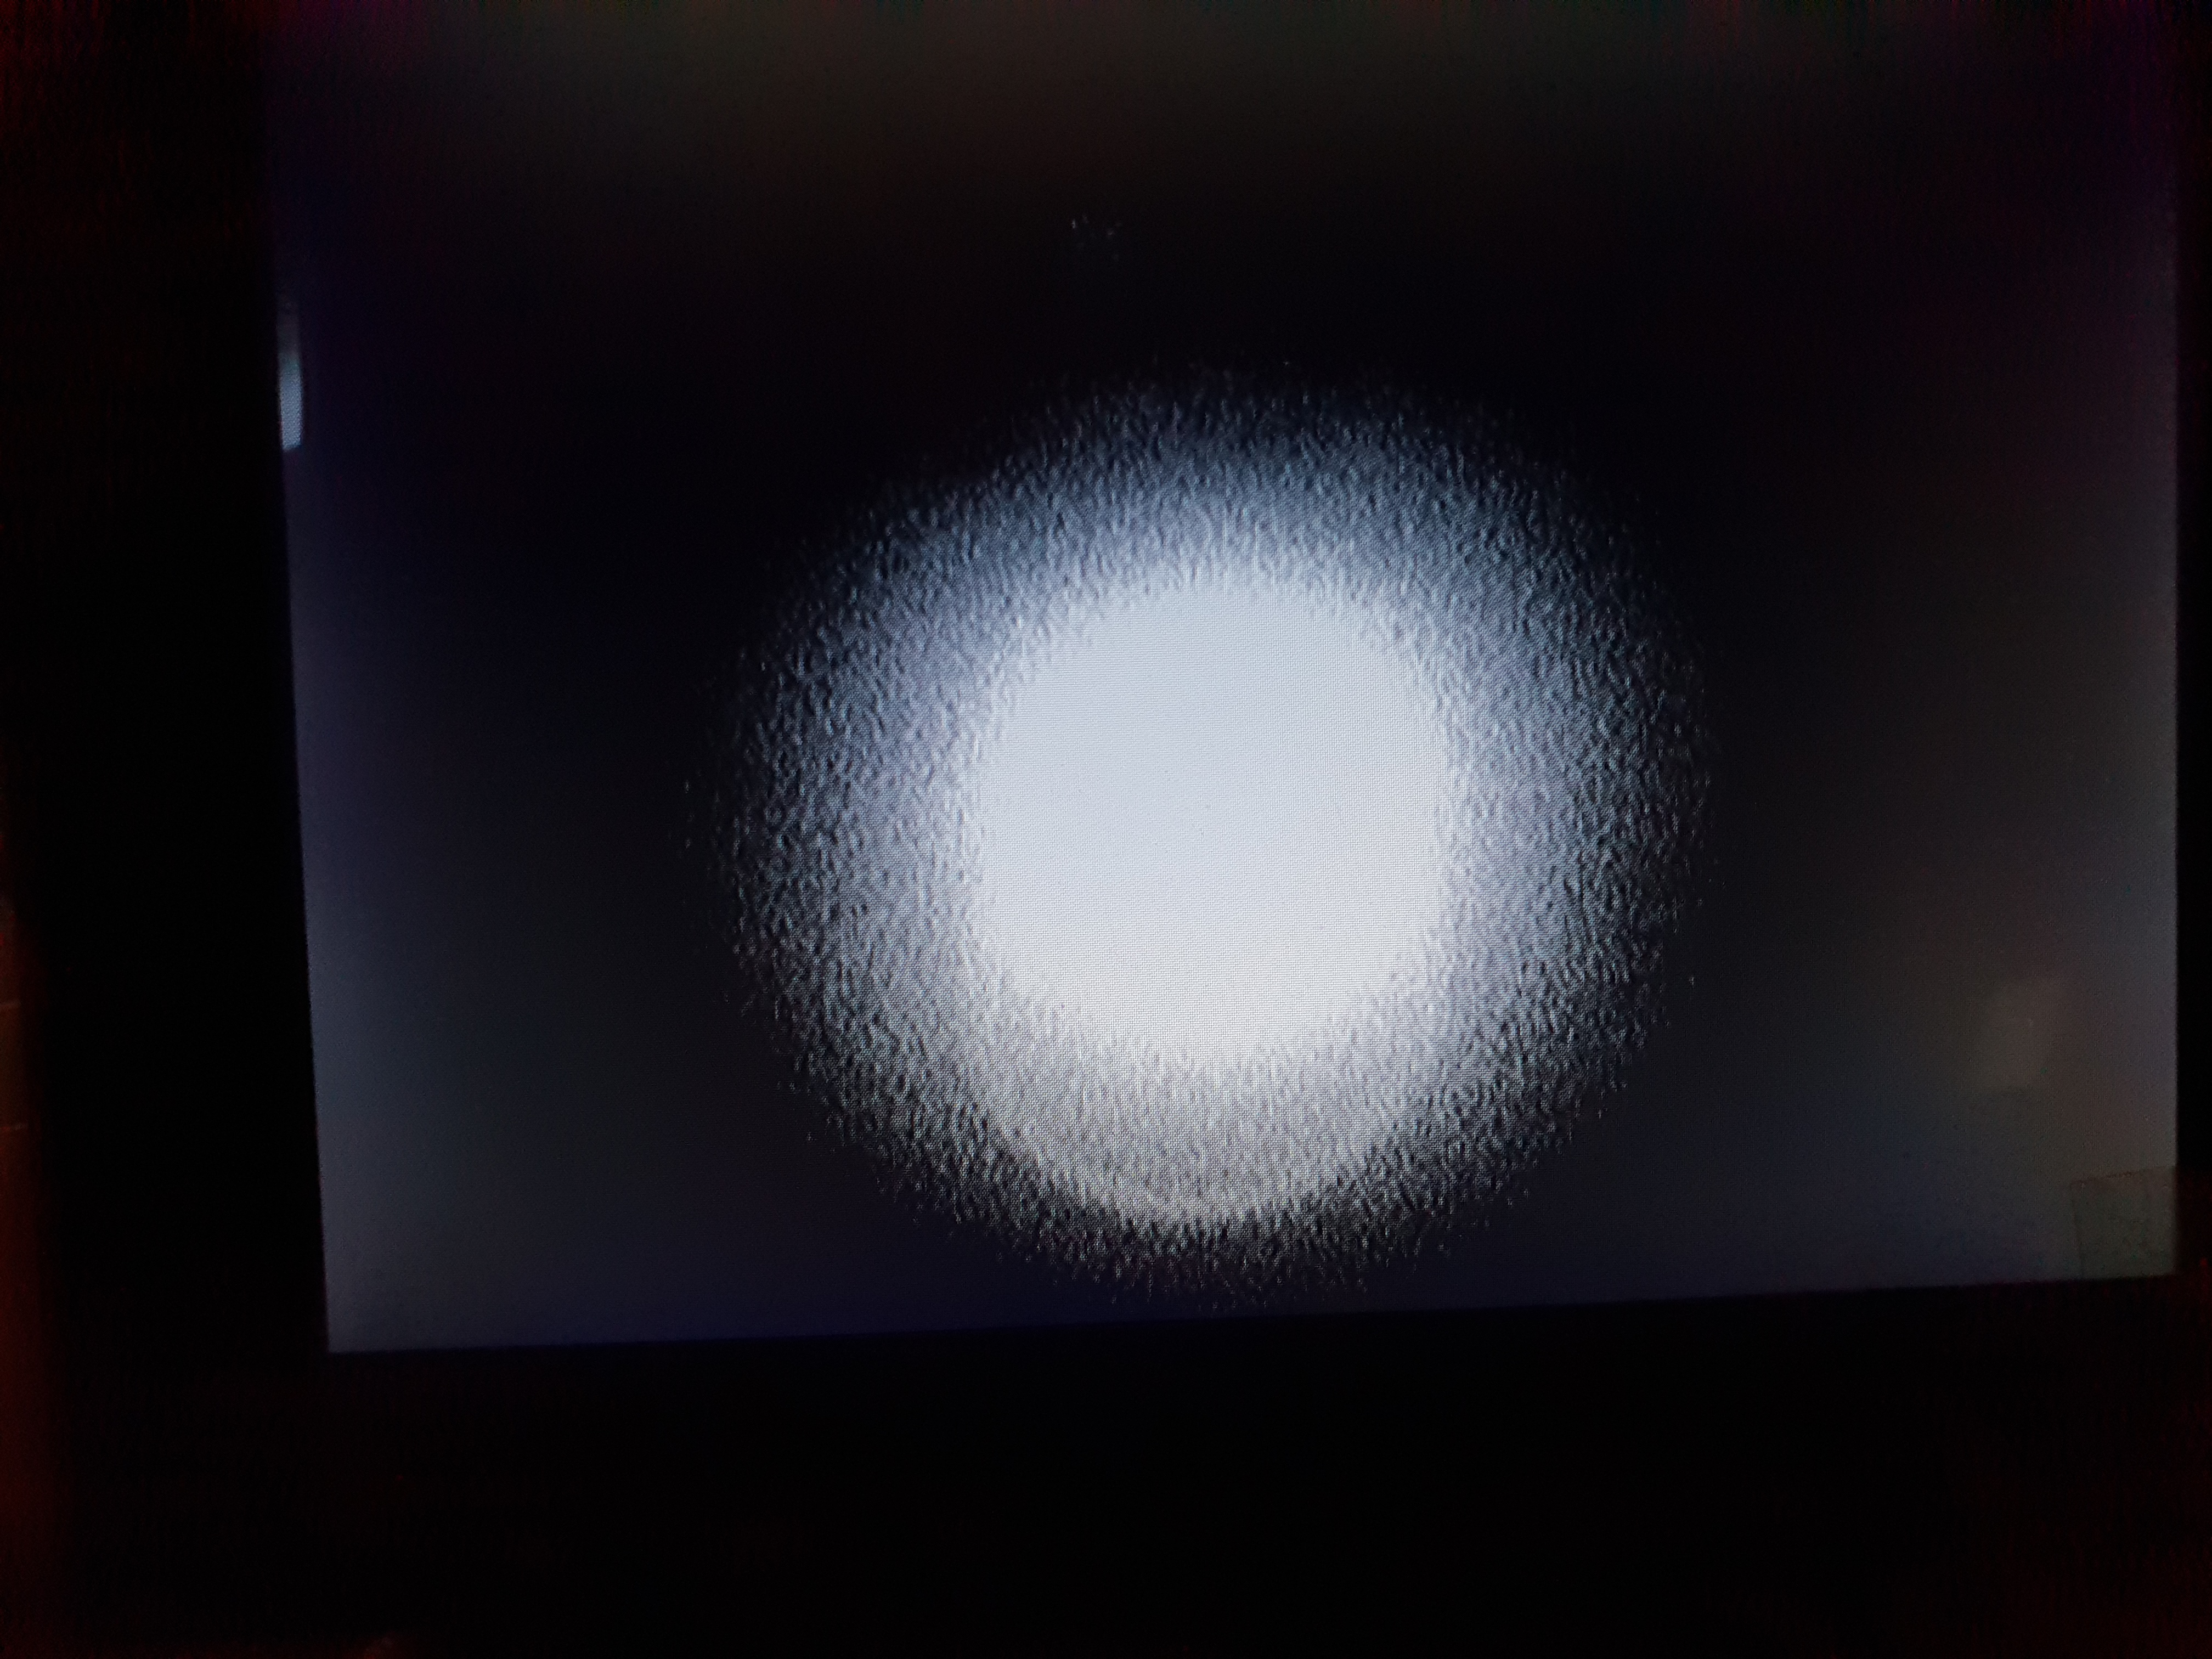
\includegraphics[width = \textwidth]{./content/images/diodelaser_lasering.jpg}
          \caption{Lasing.}
          \label{fig:lasering}
      \end{subfigure}
  \caption{Observed emission modes of the laser. The diode laser behaves like a regular
  LED under a certain current threshold, \ref{fig:not_lasering}. After reaching the
  current threshold the diode laser emits coherent light \ref{fig:lasering}. }
\label{fig: emission_modes}
\end{figure}
If the current reaches a certain threshold, the diode starts to emit coherent
light and can be used as a laser. To operate the diode laser efficiently,
the current is decreased slightly below the threshold. The light spot on the
display card is now equal to image \ref{fig:not_lasering}. By moving the knobs
on the diffraction grating carefully, the diode starts to emit coherent light -
as shown in image \ref{fig:lasering}. The knobs slightly change the length of
the external cavity and how the light reflected from the grating hits the diode.
The process is repeated as long as it is possible to get coherent light. The minimal
current is determined with a voltage measurement. With the resistance
of the current source ($\SI{100}{\ohm}$) and Ohm's law, the current can be calculated
to $I\ua{min}=\SI{0.33}{\ampere}$. As the next step, the display card has to be removed
and a rubidium gas cell is mounted into the laser path. As shown in figure~\ref{fig: positioning_cell_camera},
the camera is repositioned to record the center of the cell.
\begin{figure}
  \centering
  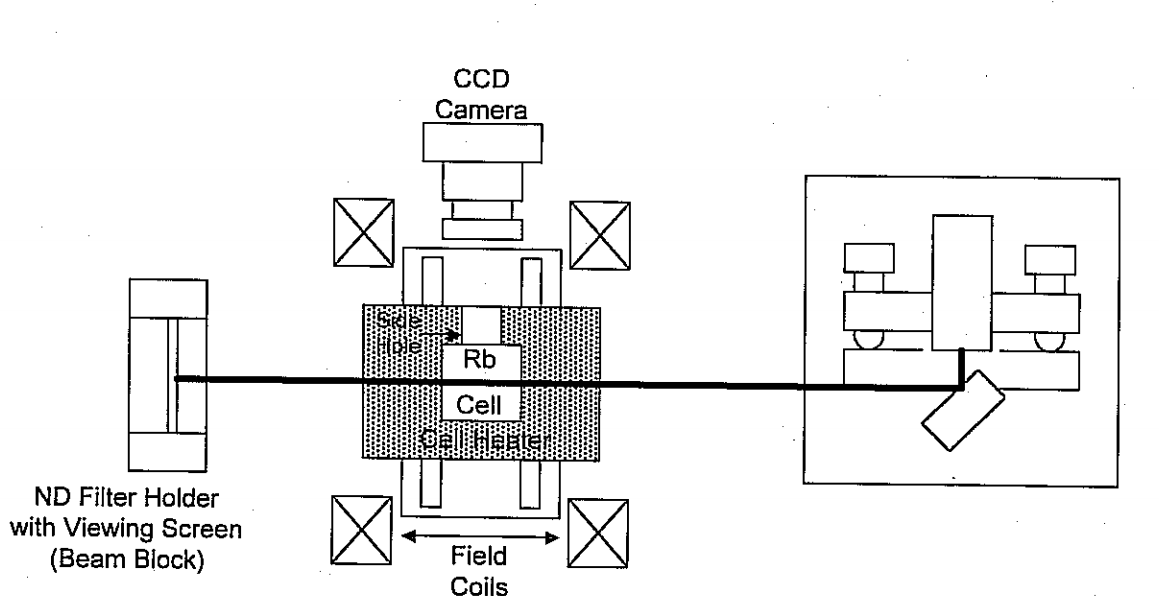
\includegraphics[width = 0.75\textwidth]{./content/images/cell_camera_heater.png}
  \caption{Positioning of cell and camera.}
  \label{fig: positioning_cell_camera}
\end{figure}
To decrease the intensity of the laser beam before entering the cell, ND filters can be used.
The diode current is increased slowly until the camera observes the fluorescence
of rubidium. Rubidium is only stimulated within the laser beam. Hence,
the characteristic fluorescence shape should be a line respective a cylinder
as demonstrated in figure~\ref{fig: fluro_rubidium}.
\begin{figure}
  \centering
  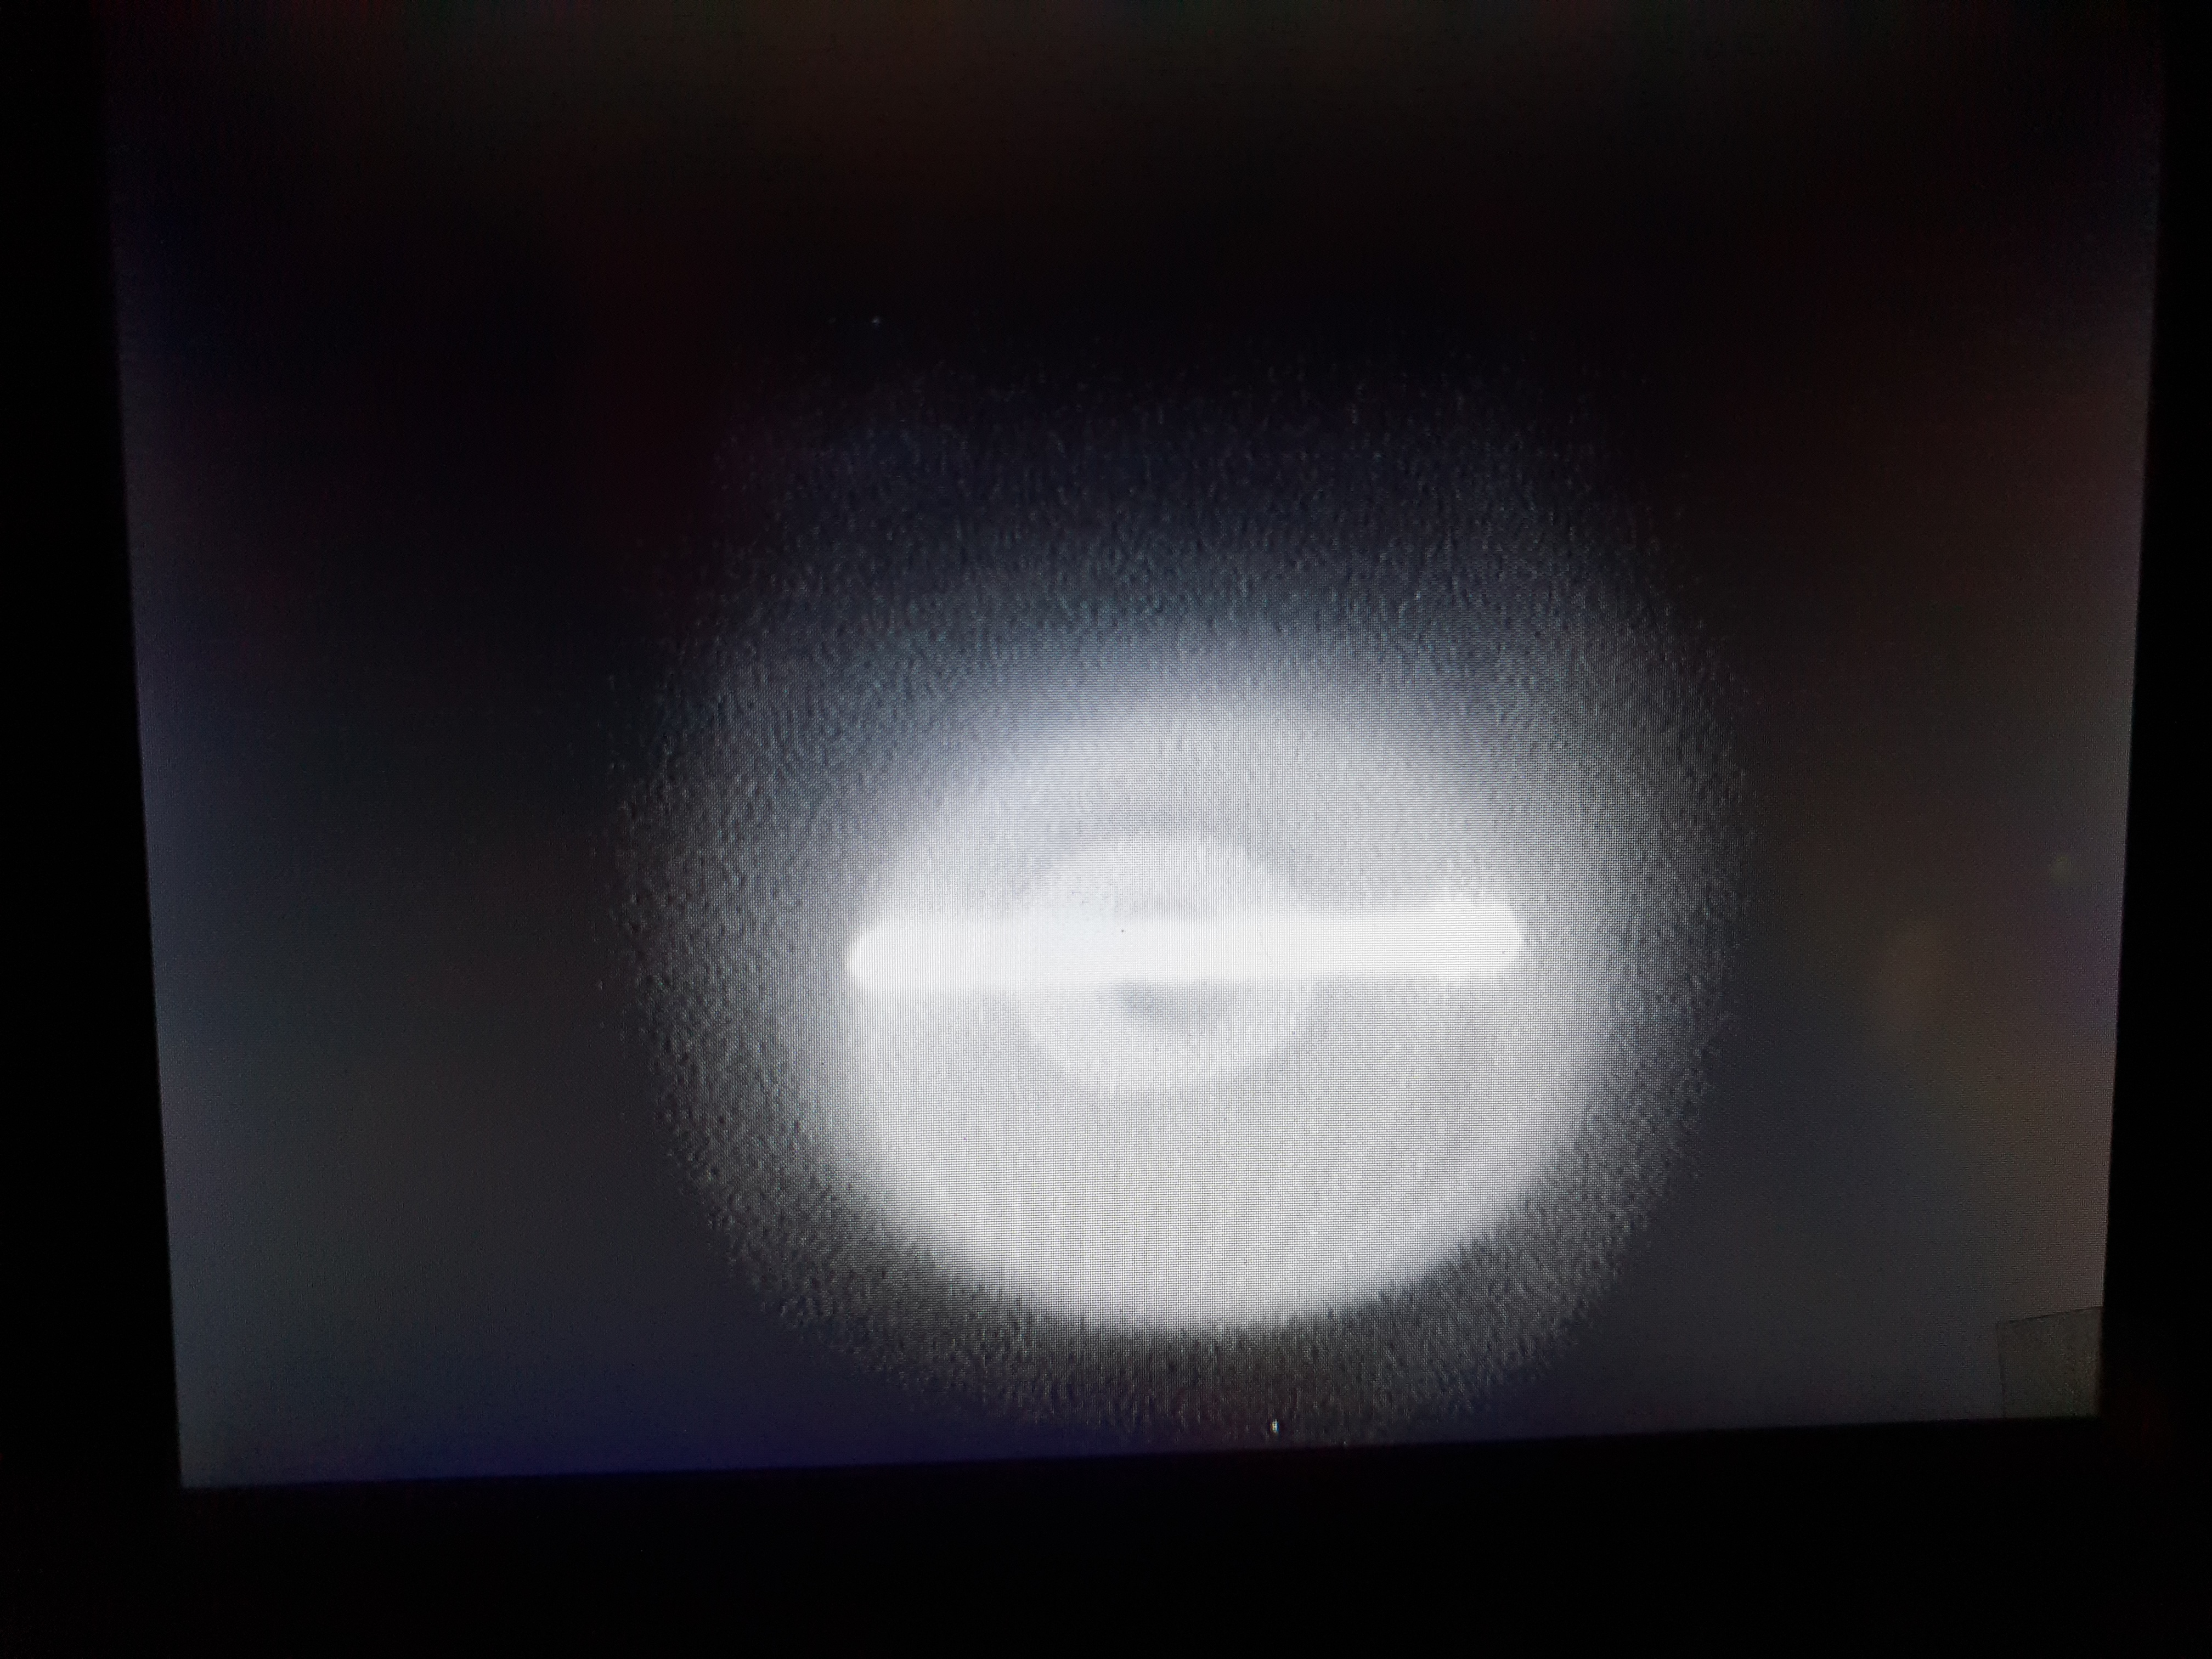
\includegraphics[width = 0.5\textwidth]{./content/images/emission_of_Ga.jpg}
  \caption{Fluorescence of rubidium (line).}
  \label{fig: fluro_rubidium}
\end{figure}

For a detailed investigation, the ramp generator is connected to the oscilloscope
and piezo controller. This makes it possible to vary the energy of the beam slightly.
Instead of the beam blocker, a photodiode is placed on the
optical table. Whenever the energy of the beam is equal to one of the rubidium
absorption energies, the beam intensity drops and can be detected as a peak.
Graph~\ref{fig: spectrum} shows such a spectrum exemplary.
\begin{figure}
  \centering
  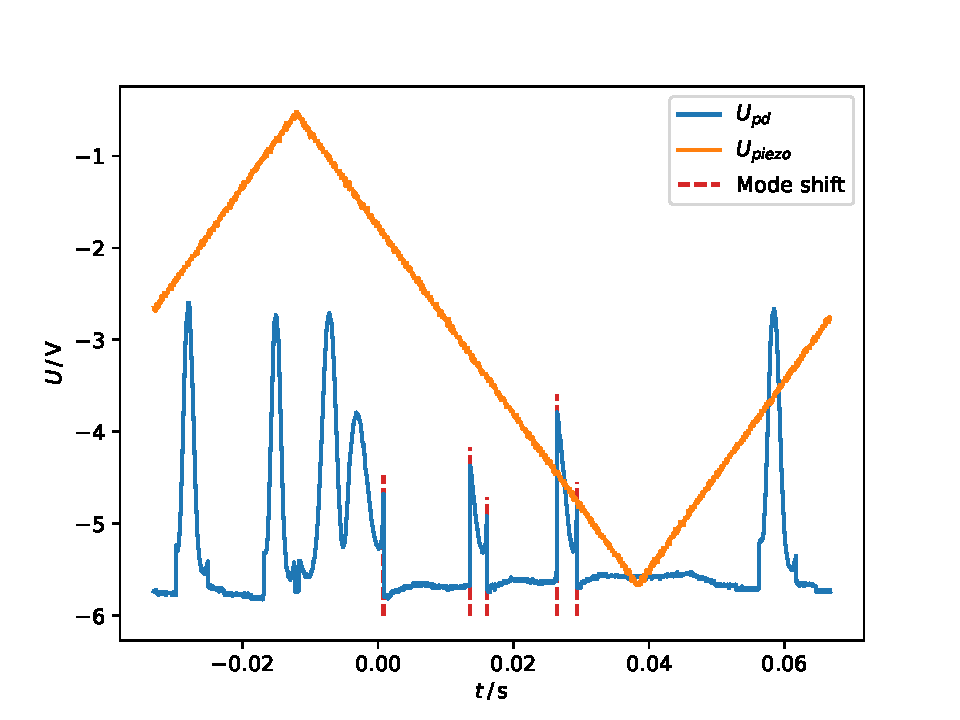
\includegraphics[width = 0.75\textwidth]{../analysis/plots/modeshift.pdf}
  \caption{Example of the spectrum measured with the photodiode. This kind of spectrum also
          shows mode hops.}
  \label{fig: spectrum}
\end{figure}
The plot also shows mode hops of the lasers, which decrease the accuracy of the
measurement. A reduction of mode hops can be achieved, when the ramp generator
controls the diode current as well. In order to shift the external and internal cavity
simultaneously. As a result of the improved experimental method, the absorption
spectrum of rubidium can be detected as shown in figure~\ref{fig: spectrum_measured}.
\begin{figure}
  \centering
  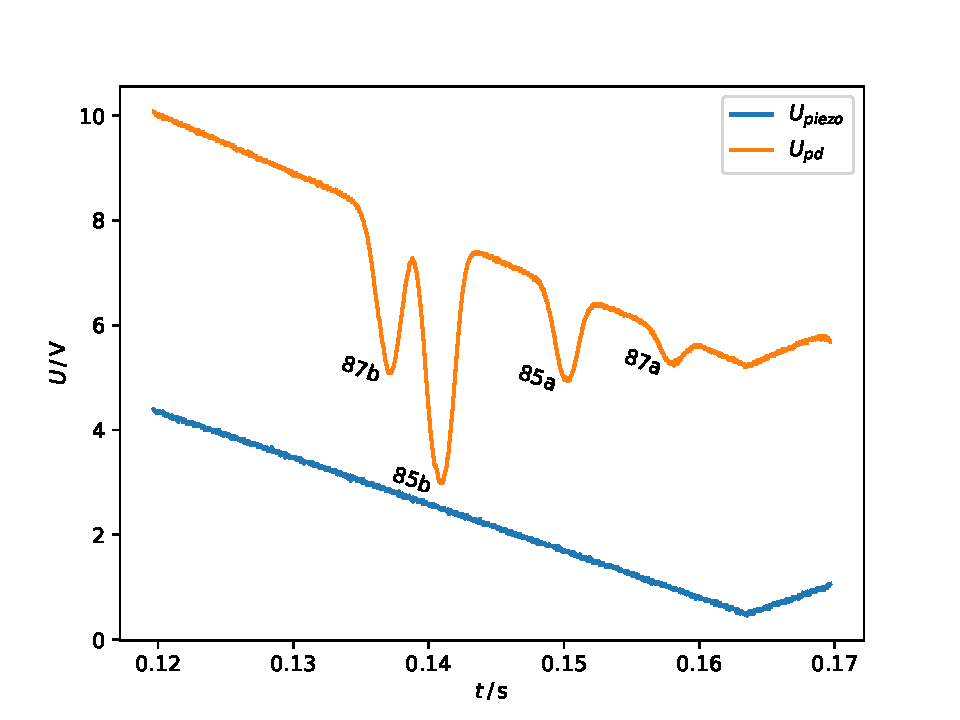
\includegraphics[width = 0.75\textwidth]{../analysis/plots/spectrum_angled.pdf}
  \caption{Measured absorption spectrum of rubidium with one photodiode.}
  \label{fig: spectrum_measured}
\end{figure}
To identify the peaks, figure~\ref{fig: spectrum_manual} was used.
\begin{figure}
  \centering
  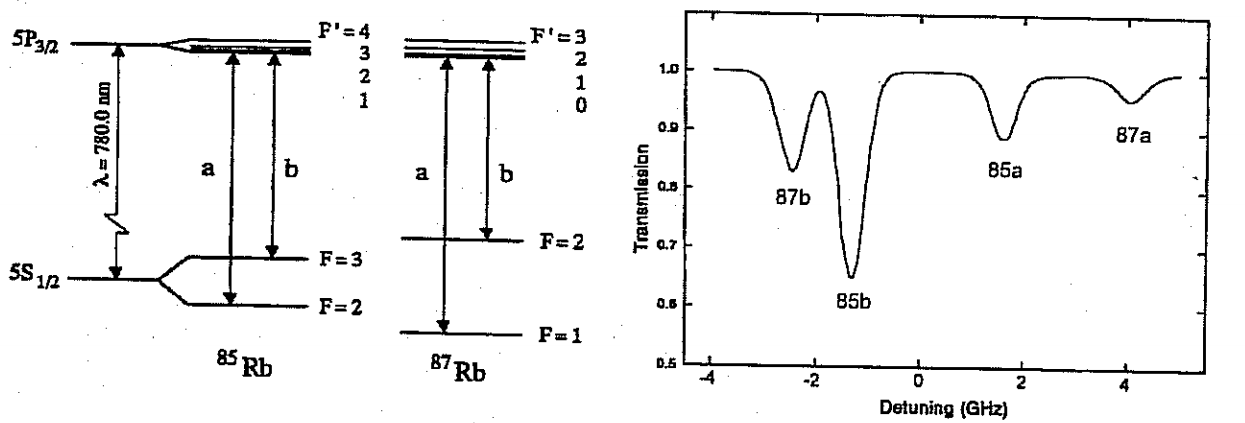
\includegraphics[width = 0.75\textwidth]{./content/images/absorption_spectrum_rubidium.png}
  \caption{Absorption spectrum of rubidium given by the manual~\cite{anleitung60}.}
  \label{fig: spectrum_manual}
\end{figure}
Finally, a second photodiode and a 50:50 beam splitter as shown in figure~\ref{fig: setup}
are used to remove the angle in the plot~\ref{fig: spectrum_measured}. The two signals of
the photodiode are subtracted. Hence, the oscilloscope only shows the
absorption spectrum of rubidium, instead of the spectrum plus the varying intensity created by the
ramp generator. The measured spectrum is shown in figure~\ref{fig: spectrum_measured_straight}.
\begin{figure}
  \centering
  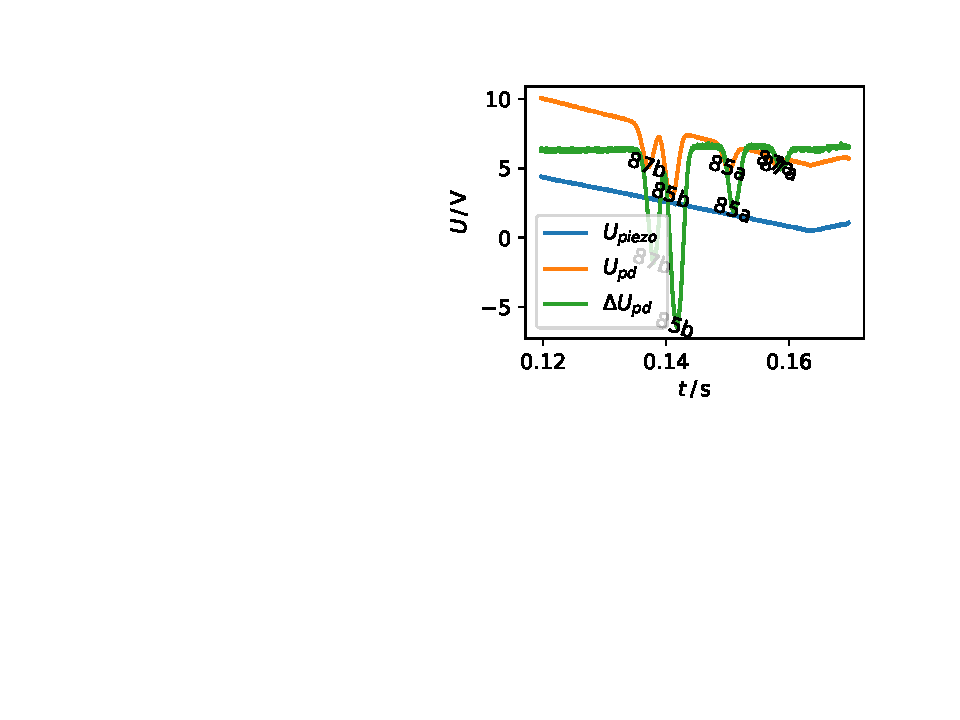
\includegraphics[width = 0.75\textwidth]{../analysis/plots/spectrum_straight.pdf}
  \caption{Measured absorption spectrum of rubidium with two photodiodes.}
  \label{fig: spectrum_measured_straight}
\end{figure}
